\documentclass[border=10pt]{standalone}
\usepackage[svgnames]{xcolor}
\usepackage{amsmath}
\usepackage{pgfplots}
\pgfplotsset{compat=newest}
\usepackage[sfdefault]{FiraSans}
\usepackage{FiraMono}
\renewcommand*\familydefault{\sfdefault}
\begin{document}
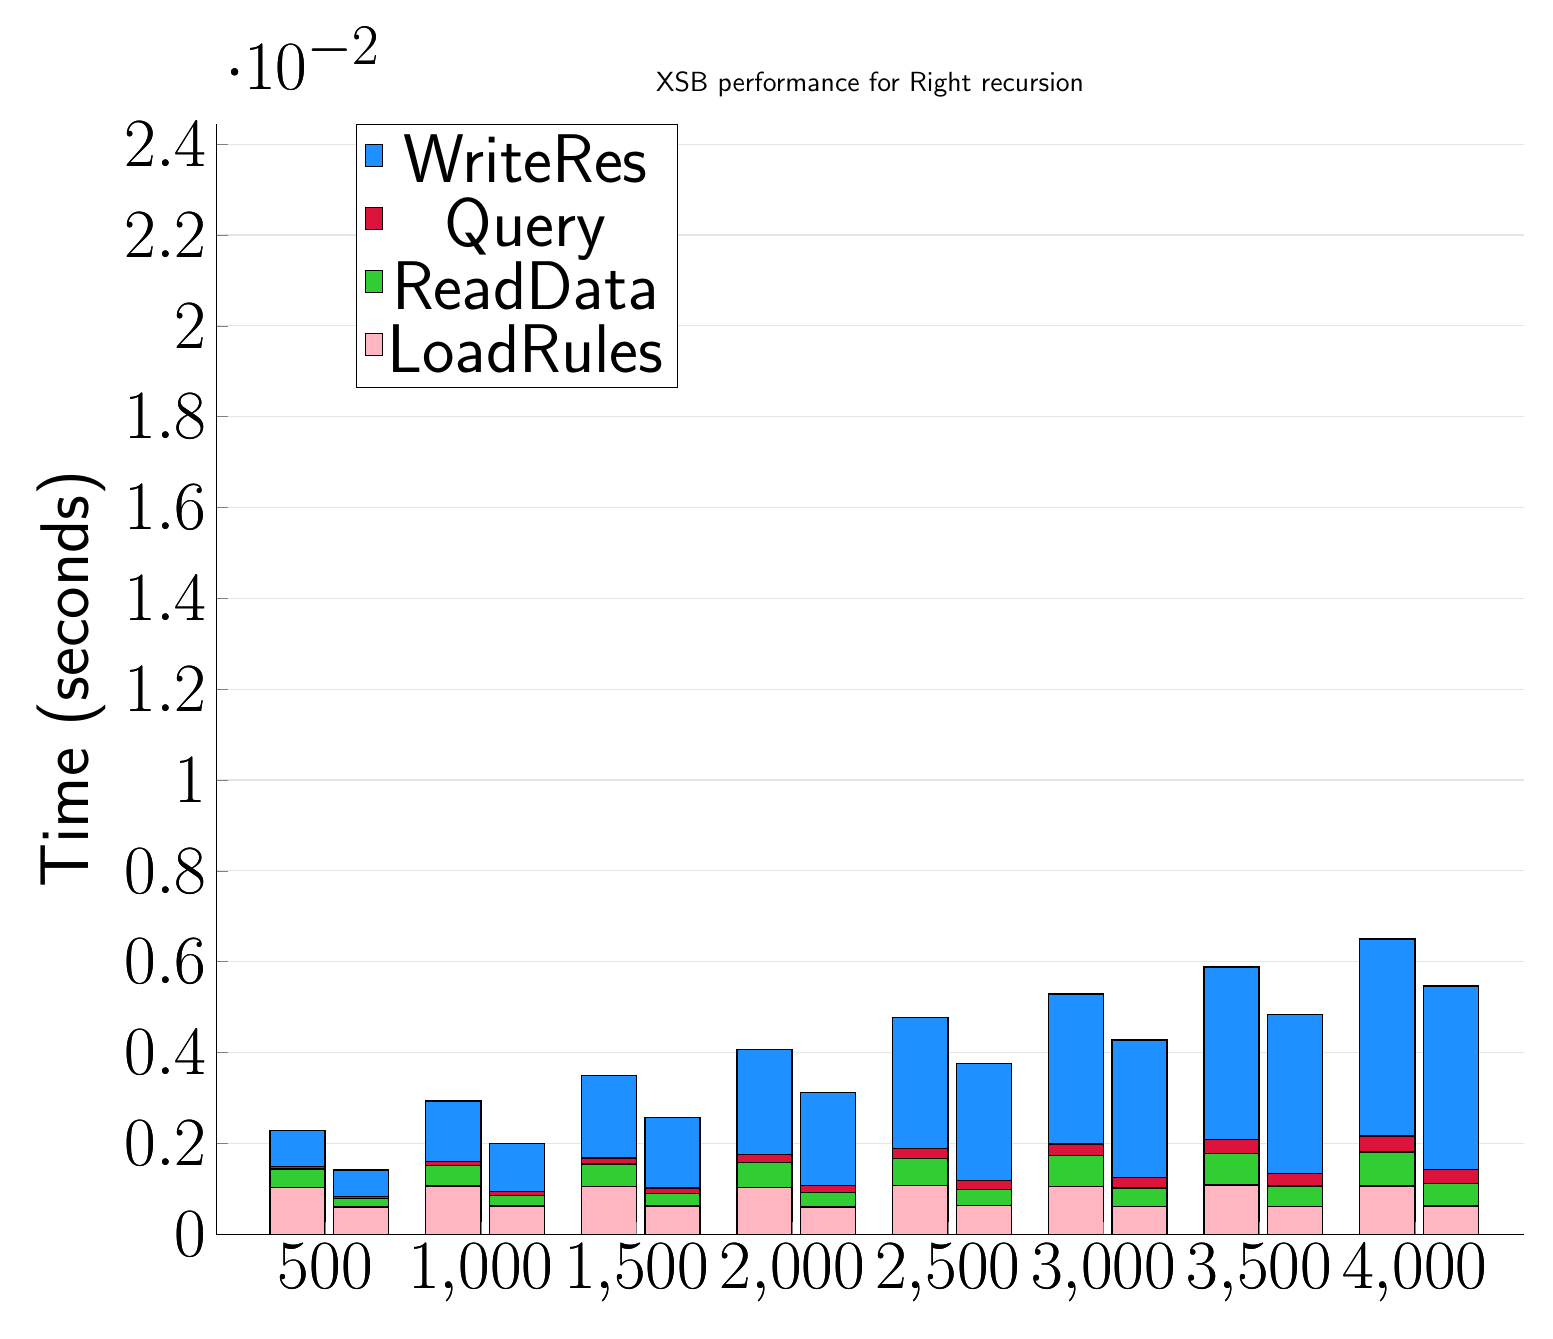
\begin{tikzpicture}
	\begin{axis}[
			ybar stacked,
			title={XSB performance for Right recursion},
			bar shift=-10pt,
			width=1.5\textwidth,
			bar width=0.7cm,
			ymajorgrids, tick align=inside,
			major grid style={draw=gray!20},
			xtick=data,
			ymin=0, ymax=0.02445413589477539,
			axis x line*=bottom,
			axis y line*=left,
			enlarge x limits=0.1,
			legend style={
					at={(0.23, 1)},
					anchor=north,
					legend columns=1,
					font=\Huge,
				},
			ylabel={Time (seconds)},
			label style={font=\Huge},
			tick label style={font=\Huge},
		]
		\addlegendimage{fill=DodgerBlue, draw=black, line width=0.2pt}
		\addlegendentry{WriteRes}
		\addlegendimage{fill=Crimson, draw=black, line width=0.2pt}
		\addlegendentry{Query}
		\addlegendimage{fill=LimeGreen, draw=black, line width=0.2pt}
		\addlegendentry{ReadData}
		\addlegendimage{fill=LightPink, draw=black, line width=0.2pt}
		\addlegendentry{LoadRules}
		\addplot +[fill=LightPink, draw=black, line width=0.5pt] coordinates {
				(500, 0.001032757759094237)
				(1000, 0.001059556007385253)
				(1500, 0.0010560989379882811)
				(2000, 0.0010342359542846668)
				(2500, 0.0010780811309814438)
				(3000, 0.0010509967803955067)
				(3500, 0.001079702377319336)
				(4000, 0.0010615587234497081)
			};
		\addplot +[fill=LimeGreen, draw=black, line width=0.5pt] coordinates {
				(500, 0.00040497779846191426)
				(1000, 0.00045316219329833975)
				(1500, 0.00048761367797851564)
				(2000, 0.0005454063415527344)
				(2500, 0.0005912303924560548)
				(3000, 0.0006817817687988281)
				(3500, 0.0006981372833251953)
				(4000, 0.000750565528869629)
			};
		\addplot +[fill=Crimson, draw=black, line width=0.5pt] coordinates {
				(500, 5.509853363037109e-05)
				(1000, 9.49382781982422e-05)
				(1500, 0.0001329660415649413)
				(2000, 0.00017480850219726553)
				(2500, 0.0002140283584594726)
				(3000, 0.0002552509307861327)
				(3500, 0.0003029108047485352)
				(4000, 0.00035035610198974593)
			};
		\addplot +[fill=DodgerBlue, draw=black, line width=0.5pt] coordinates {
				(500, 0.0007919073104858398)
				(1000, 0.0013286828994750967)
				(1500, 0.0018146514892578142)
				(2000, 0.002316641807556152)
				(2500, 0.002884793281555176)
				(3000, 0.0033028125762939453)
				(3500, 0.0038050889968872063)
				(4000, 0.004333639144897461)
			};
	\end{axis}
	\begin{axis}[
			ybar stacked,
			bar shift=13pt,
			width=1.5\textwidth,
			bar width=0.7cm,
			ymajorgrids, tick align=inside,
			major grid style={draw=none},
			xtick=data,
			ymin=0, ymax=0.02445413589477539,
			axis x line*=none,
			axis y line*=none,
			enlarge x limits=0.1,
			label style={font=\Huge},
			tick label style={font=\Huge},
		]
		\addplot +[fill=LightPink, draw=black, line width=0.5pt] coordinates {
				(500, 0.0006004999999999998)
				(1000, 0.0006172999999999999)
				(1500, 0.0006217)
				(2000, 0.0006018999999999996)
				(2500, 0.0006263999999999998)
				(3000, 0.0006061000000000004)
				(3500, 0.0006072000000000002)
				(4000, 0.0006170000000000004)
			};
		\addplot +[fill=LimeGreen, draw=black, line width=0.5pt] coordinates {
				(500, 0.0001870999999999996)
				(1000, 0.00023640000000000003)
				(1500, 0.0002747000000000001)
				(2000, 0.00031480000000000033)
				(2500, 0.0003638999999999998)
				(3000, 0.0004104999999999994)
				(3500, 0.0004536999999999996)
				(4000, 0.0005014999999999996)
			};
		\addplot +[fill=Crimson, draw=black, line width=0.5pt] coordinates {
				(500, 4.9300000000000385e-05)
				(1000, 8.680000000000005e-05)
				(1500, 0.0001227999999999997)
				(2000, 0.0001572999999999997)
				(2500, 0.0001942000000000002)
				(3000, 0.00022899999999999998)
				(3500, 0.00027290000000000013)
				(4000, 0.00030709999999999977)
			};
		\addplot +[fill=DodgerBlue, draw=black, line width=0.5pt] coordinates {
				(500, 0.0005741999999999995)
				(1000, 0.0010583)
				(1500, 0.0015447)
				(2000, 0.0020427000000000006)
				(2500, 0.0025710999999999998)
				(3000, 0.0030288999999999997)
				(3500, 0.0035095999999999994)
				(4000, 0.004040500000000001)
			};
	\end{axis}
\end{tikzpicture}

\end{document}
